\documentclass[12pt, twoside]{article}
\documentclass[12pt, twoside]{article}
\usepackage[letterpaper, margin=1in, headsep=0.2in]{geometry}
\setlength{\headheight}{0.6in}
%\usepackage[english]{babel}
\usepackage[utf8]{inputenc}
\usepackage{microtype}
\usepackage{amsmath}
\usepackage{amssymb}
%\usepackage{amsfonts}
\usepackage{siunitx} %units in math. eg 20\milli\meter
\usepackage{yhmath} % for arcs, overparenth command
\usepackage{tikz} %graphics
\usetikzlibrary{quotes, angles}
\usepackage{graphicx} %consider setting \graphicspath{{images/}}
\usepackage{parskip} %no paragraph indent
\usepackage{enumitem}
\usepackage{multicol}
\usepackage{venndiagram}

\usepackage{fancyhdr}
\pagestyle{fancy}
\fancyhf{}
\renewcommand{\headrulewidth}{0pt} % disable the underline of the header
\raggedbottom
\hfuzz=2mm %suppresses overfull box warnings

\usepackage{hyperref}

\title{PreCalculus}
\author{Chris Huson}
\date{May 2023}

\fancyhead[LE]{\thepage}
\fancyhead[RO]{\thepage \\ Name: \hspace{3cm} \,\\}
\fancyhead[LO]{BECA / Huson / Unit 12: Integral Calculus \\* 25 May 2023}

\begin{document}

\subsubsection*{12.12 Final Exam: Differential and Integral calculus}
\begin{enumerate}

\item Find the derivative of each polynomial function.
\begin{enumerate}
    \begin{multicols}{2}
    \item $f(x)=x^2+7x$ \\[0.2cm]
    $\displaystyle \frac{dy}{dx}=$ \vspace{1cm}
    \item $f(x)=x^3+\frac{1}{2}x^2-9$\\[0.2cm]
    $\displaystyle \frac{dy}{dx}=$ \vspace{1cm}
  \end{multicols} 
\end{enumerate} \vspace{1cm}

\item Evaluate the function and its derivative for a given value of $x$.\\[0.3cm] 
  Given $f(x)=5x^2+x$
  \begin{enumerate}[itemsep=2cm]
    \item Find $f(2)$
    \item Find $f'(x)$
    \item Find $f'(2)$
  \end{enumerate} \vspace{3cm}

\item Find the anti-derivative of each polynomial function (include the constant of integration)
  \begin{enumerate}
    \begin{multicols}{2}
    \item $f(x)=3x^2+5$ \\[0.2cm]
    $F(x)=$ \vspace{1cm}
    \item $f(x)=16x^3+6x^2-2x$\\[0.2cm]
    $F(x)=$ \vspace{1cm}
  \end{multicols} 
  \end{enumerate} \vspace{1cm}

\newpage
\item The graph shows the polynomial function $\displaystyle y=x^3+2x^2-2x-2$. Its derivative is $\displaystyle \frac{dy}{dx}=3x^2+4x-2$. 
  \begin{multicols}{2}
    \begin{enumerate}
        \item Write down the coordinates of $P$. \vspace{1cm}
        \item Find the slope of the tangent at $P$. \vspace{2cm}
        \item Write down the equation of the tangent line through $P$. \vspace{1.5cm}
        \item Draw the tangent line on the graph accurately with a straight edge.
    \end{enumerate}
        \begin{center}
    \begin{tikzpicture}[x=1cm, y=1cm, scale=1]
        \draw [thin, color=lightgray, xstep=1.0cm,ystep=1.0cm] (-4,-4.1) grid (3,4);
        \draw [thick, ->] (-4,0) -- (+3.3,0) node [above left]{$x$};
        \draw [thick, ->] (0,-4.2) -- (0,4.2) node [right]{$y$};
        \foreach \x in {-4,...,3}
            \draw (\x cm,0) -- (\x cm,0) node[below] {$\x$};
        \foreach \y in {-4,...,4}
            \draw[shift={(0,\y)}] (2pt,0pt)--(-2pt,0pt) node[left]{$\y$};
        \draw [thick,<->,smooth,domain=-2.9:1.5] plot(\x,{(\x*\x*\x+2*\x*\x-2*\x-2)});
        \fill (1,-1) circle[radius=0.07] node[below left]{$P$};
    \end{tikzpicture}
    \end{center}
\end{multicols}

\item The function $y=-x^{2}+3x+2$ is graphed on the grid below. Find its derivative and the equations of the tangent and normal lines through point $(1,4)$. Draw the lines.
    \begin{flushright}
        \begin{tikzpicture}[x=1cm, y=1cm, scale=0.9]
            \draw [thin, color=lightgray, xstep=1.0cm,ystep=1.0cm] (-2,-2) grid (5,7);
            \draw [thick, ->] (-2,0) -- (+5.3,0) node [above right]{$x$};
            \draw [thick, ->] (0,-2.3) -- (0,7.3) node [right]{$y$};
            \foreach \x in {-2,...,5}
                \draw (\x cm,0) -- (\x cm,0) node[below] {$\x$};
            \foreach \y in {-2,...,7}
                \draw[shift={(0,\y)}] (2pt,0pt)--(-2pt,0pt) node[left]{$\y$};
            \draw [thick,<->,smooth,domain=-1.1:4.1] plot(\x,{(-\x*\x+3*\x+2)});
        \end{tikzpicture}
    \end{flushright}

\newpage
\item A portion of the function $f(x)=5-\frac{1}{2}x$ is plotted below.
  \begin{enumerate}
    \item Write down a definite integral that represents the area of the shaded region $\mathbf{R}$. \vspace{1.5cm}
    \item Calculate the area using geometric formulas.
      \begin{flushright}
        \begin{tikzpicture}[xscale=1,yscale=1]
          \draw [thick, ->] (0,0) -- (4.5,0) node [below] {$x$};
          \draw [thick, ->] (0,0) -- (0,5.5) node [left] {$y$};
          \draw[thick, domain=2:4] plot[samples=100](\x, 5-0.5*\x);
          \draw[dashed] (2, -.15)node[below]{$2$} --(2,4);
          \draw[dashed] (4, -.15)node[below]{$4$} --(4,3);
          \fill[gray,opacity=.3] (2,0)--plot[domain=2:4](\x, 5-0.5*\x)--(4,0);
          \draw (3,2) node {$\mathbf{R}$};
        \end{tikzpicture}
      \end{flushright}
    \item Find the area using a definite integral and the methods of calculus. \vspace{2cm}
  \end{enumerate}

\newpage
    \item Part of the graph of $f(x)=-4x^3+16x$ is shown in the following diagram.
    \begin{center}
      \begin{tikzpicture}[xscale=1.2,yscale=0.3]
        \draw [thick, ->] (-1,0) -- (3.5,0) node [below] {$x$};
        \draw [thick, ->] (0,-2) -- (0,13) node [left] {$y$};
        \draw[thick, domain=-0.1:2.05] plot[samples=100](\x, {-4*(\x)^3+16*\x});
        \foreach \x in {1,2,3}
          \draw (\x cm,-0.5) -- (\x cm,0.5) node[xshift=-0.1cm,yshift=-0.6cm] {$\x$};
      \end{tikzpicture}
    \end{center}
  \begin{enumerate}
    \item Write down the antiderivative of $f(x)$. Include the constant of integration. \vspace{2cm}
    \item Write down a definite integral that represents the area of the region enclosed by the graph of $f$ and the $x$-axis from $x=0$ to $x=2$. \vspace{1.5cm}
    \item Find the area of that region using the antiderivative and applying the fundamental theorem of calculus.
  \end{enumerate}

\newpage
\subsubsection*{Calculator section}

\item The following diagram shows part of the graph of $f(x)=x^2$.
    \begin{center}
    \begin{tikzpicture}[xscale=2,yscale=1]
        \draw [thick, ->] (0,0) -- (2.8,0) node [below] {$x$};
        \draw [thick, ->] (0,-1) -- (0,6) node [left] {$y$};
        \draw[thick, domain=0:2.4] plot[samples=100](\x, {(\x)^2});
        \draw[thick] (1, -.15)node[below]{$1$} --(1,1);
        \draw[thick] (2.3, -.15)node[below]{$a$} --(2.3,2.3^2);
        \fill[gray,opacity=.3] (1,0)--plot[domain=1:2.3](\x, {\x*\x})--(2.3,0);
        \draw (1.7,1) node {$\mathbf{R}$};
    \end{tikzpicture}
    \end{center}
    \begin{enumerate}
    \item Find $\displaystyle \int_0^1 f(x) \,\mathrm{d}x$ \vspace{3cm}

    \item The shaded region $R$ is enclosed by the graph of $f$, the $x$-axis, and the lines $x=1$ and $x=a$. Find the value of $a$ so that $R \approx 4$.
  \end{enumerate}

\newpage




\end{enumerate}
\end{document}



